\documentclass{book}
\usepackage[left=2cm, right=2cm, top=2cm, bottom=2cm]{geometry}

\usepackage[spanish]{babel}
\usepackage[utf8]{inputenc}

\usepackage{pdfpages}
\usepackage[pdftex,pdfpagelabels=true,bookmarks=true]{hyperref} % Para enlaces y metadatos
\usepackage{bookmark}
\usepackage{fontawesome5}
\usepackage{fancyhdr}
\usepackage{titletoc}

\hypersetup{
    colorlinks=true,
    linkcolor=black,  % Color de los enlaces internos (por ejemplo, dentro de la tabla de contenidos)
    urlcolor=magenta,   % Color de los enlaces a URLs
    %%citecolor=green,
    pdfauthor={Moisés Serrano Samudio},
    pdftitle={Villancicos Populares},
    pdfsubject={Partituras},
    pdfkeywords={violín, trío, villancicos, navidad}
}

\title{Villancicos Populares}
\author{Moisés Serrano Samudio}
\date{\today}

\begin{document}

\newcommand{\CoverName}{Portada}%
\pagestyle{empty}%
\renewcommand{\thepage}{\CoverName}
\includepdf[pages=-]{../extend/0-portada.pdf}

\renewcommand{\CoverName}{Portadilla}%
\pagestyle{empty}%
\renewcommand{\thepage}{\CoverName}
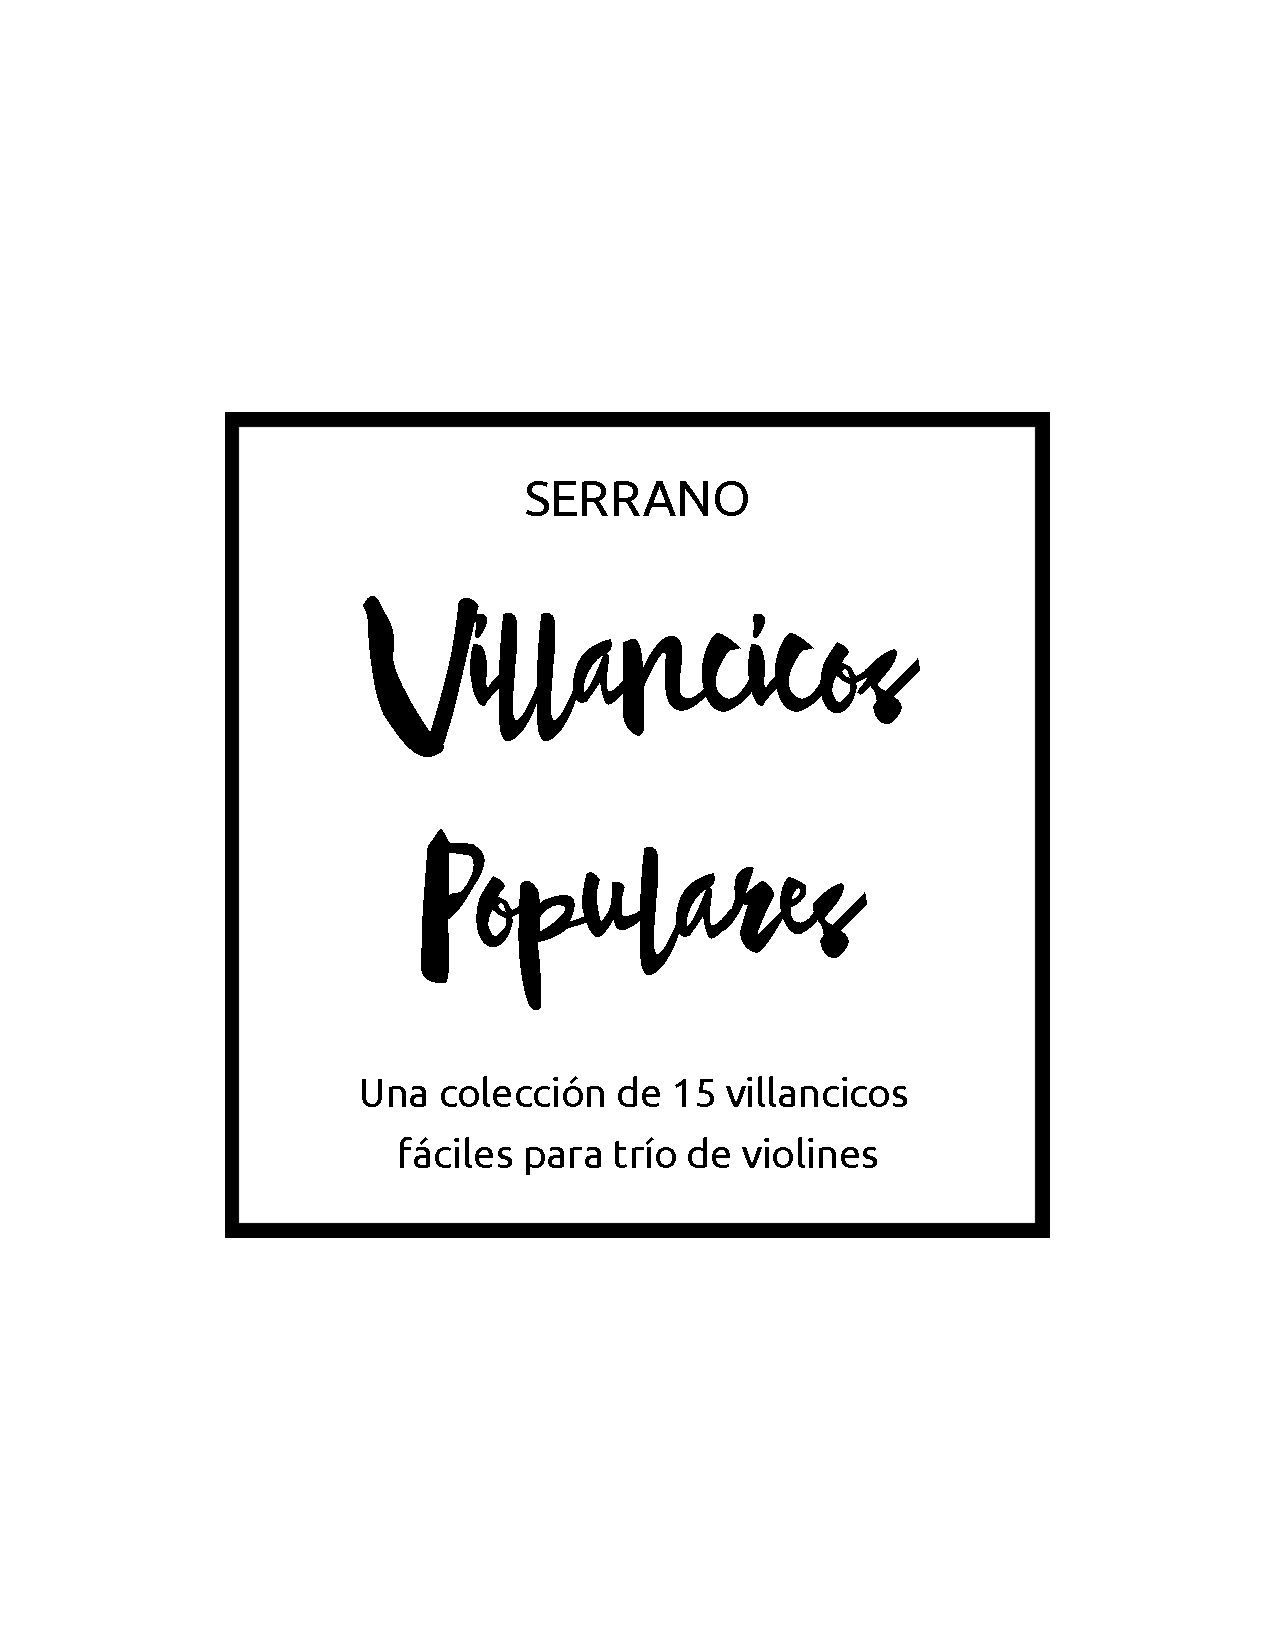
\includepdf[pages=-]{../extend/1-portadilla.pdf}

\renewcommand{\CoverName}{Licencia}%
\pagestyle{empty}%
\renewcommand{\thepage}{\CoverName}
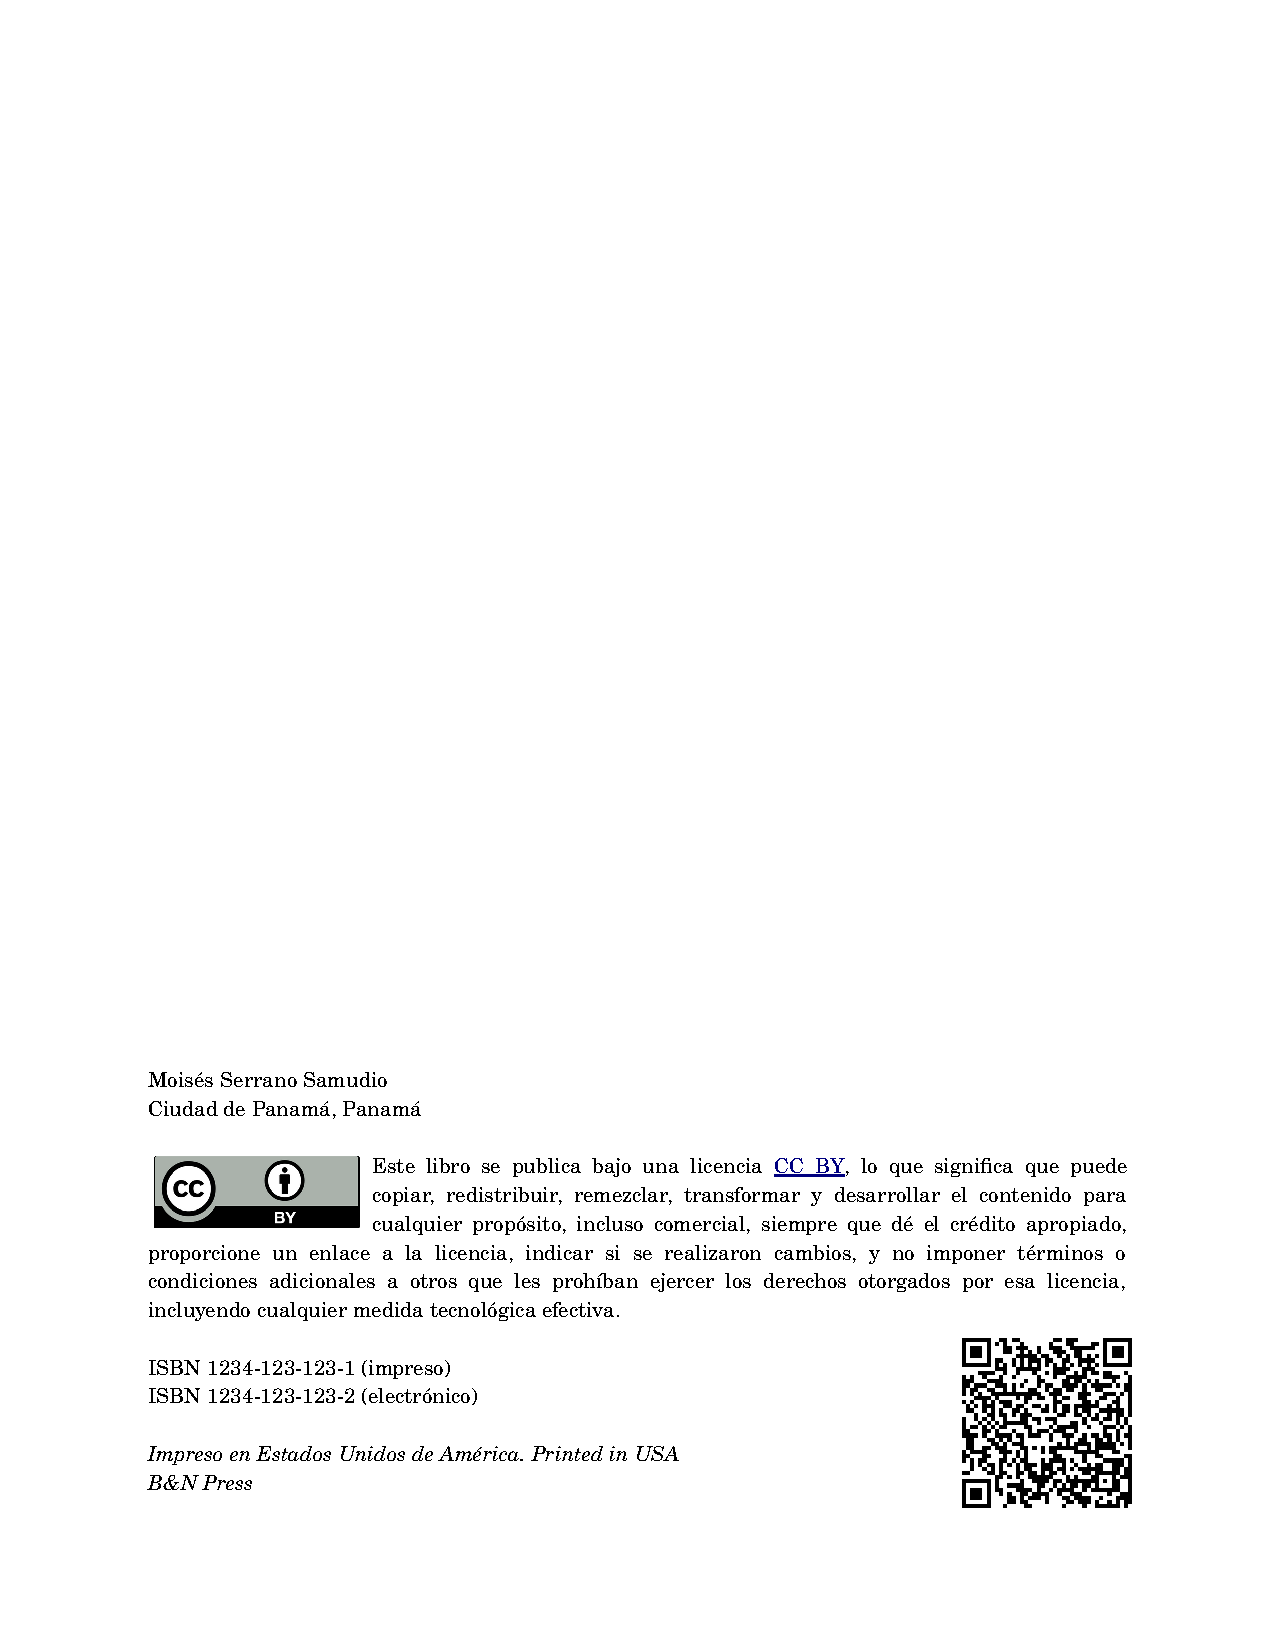
\includepdf[pages=-]{../extend/2-licencia.pdf}

\pagenumbering{roman}

%% Tabla de contenidos
\renewcommand{\contentsname}{Índice de Partituras} %% Índice de partituras
% Establecer los márgenes de la página de índice
\newgeometry{left=5cm, right=5cm, top=2cm, bottom=2cm}
\pdfbookmark{\contentsname}{Partituras}
\tableofcontents
\restoregeometry 
% Volver a ajustar los márgenes después de índice a los originales


\includepdf[pages=-]{../extend/blank.pdf}
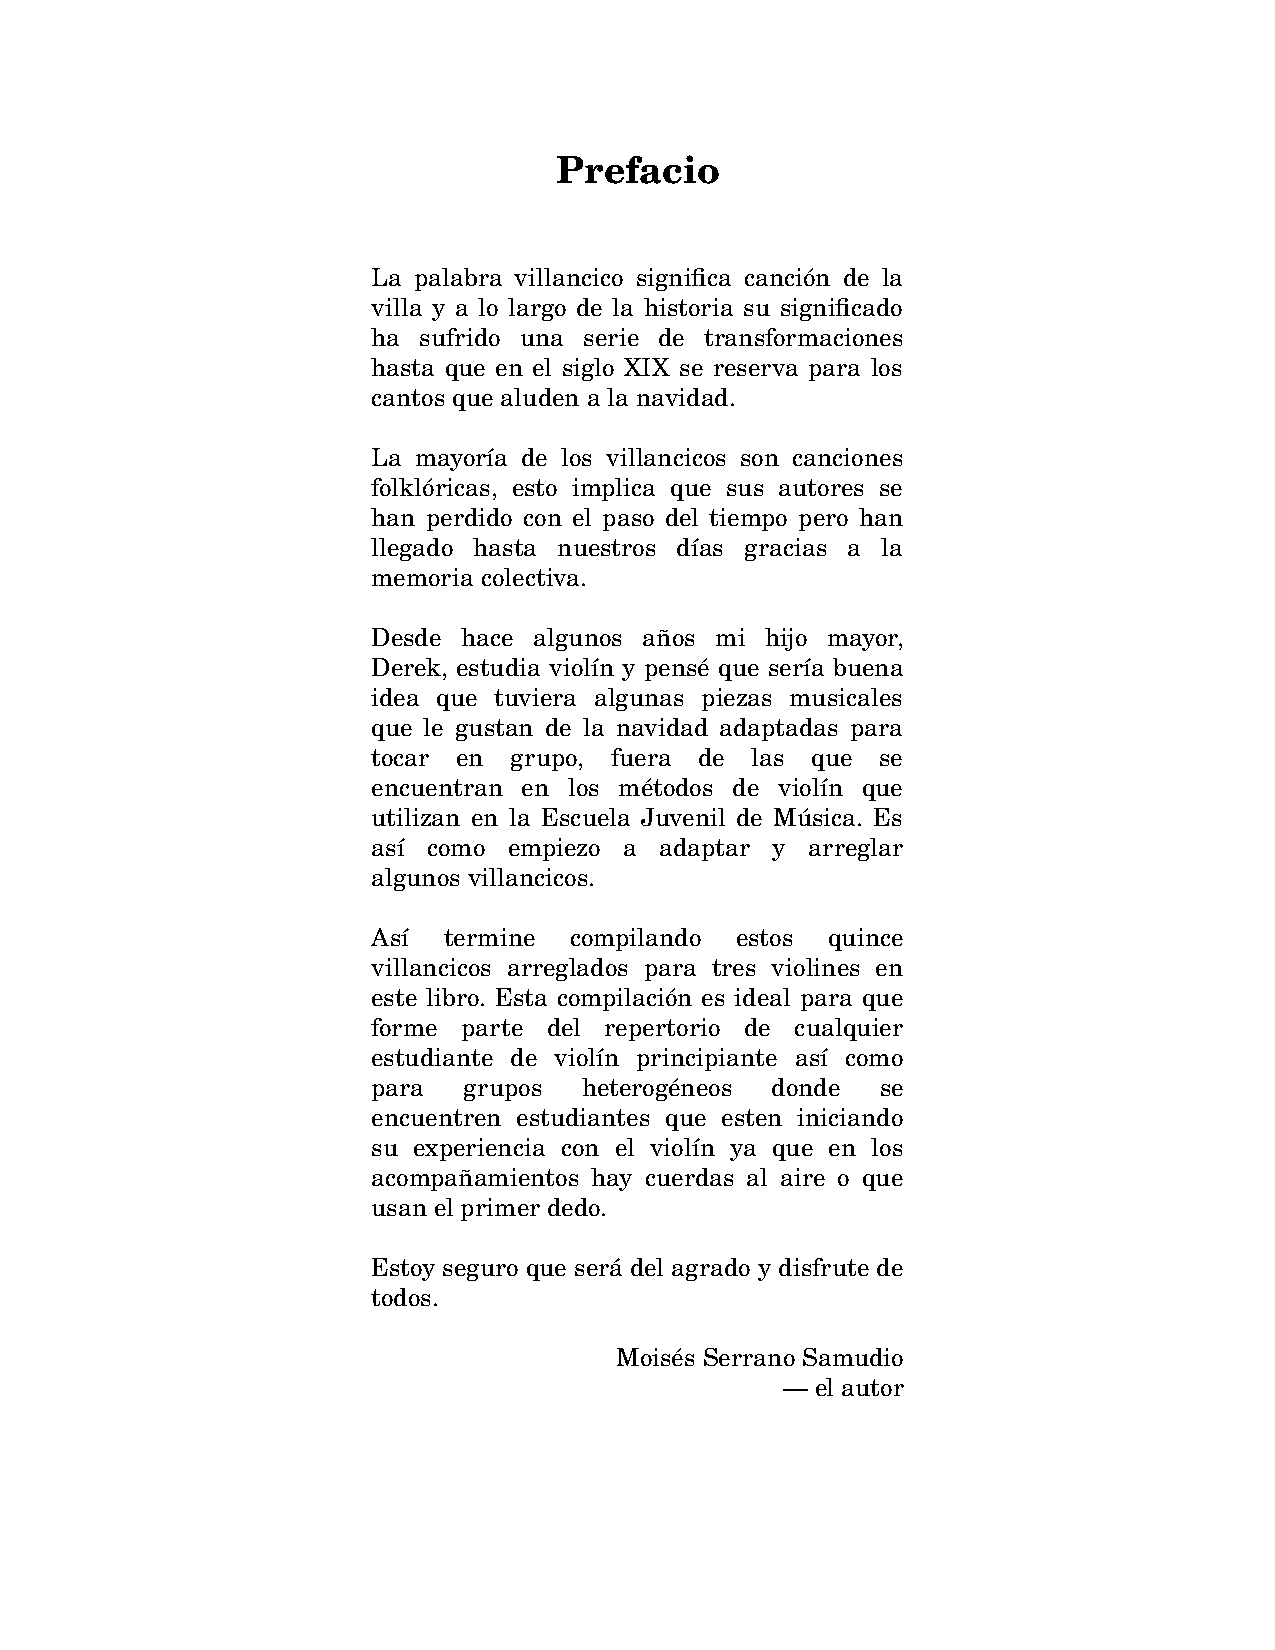
\includepdf[pages=-]{../extend/3-prefacio.pdf}

\includepdf[pages=-]{../extend/blank.pdf}

\pagenumbering{arabic}

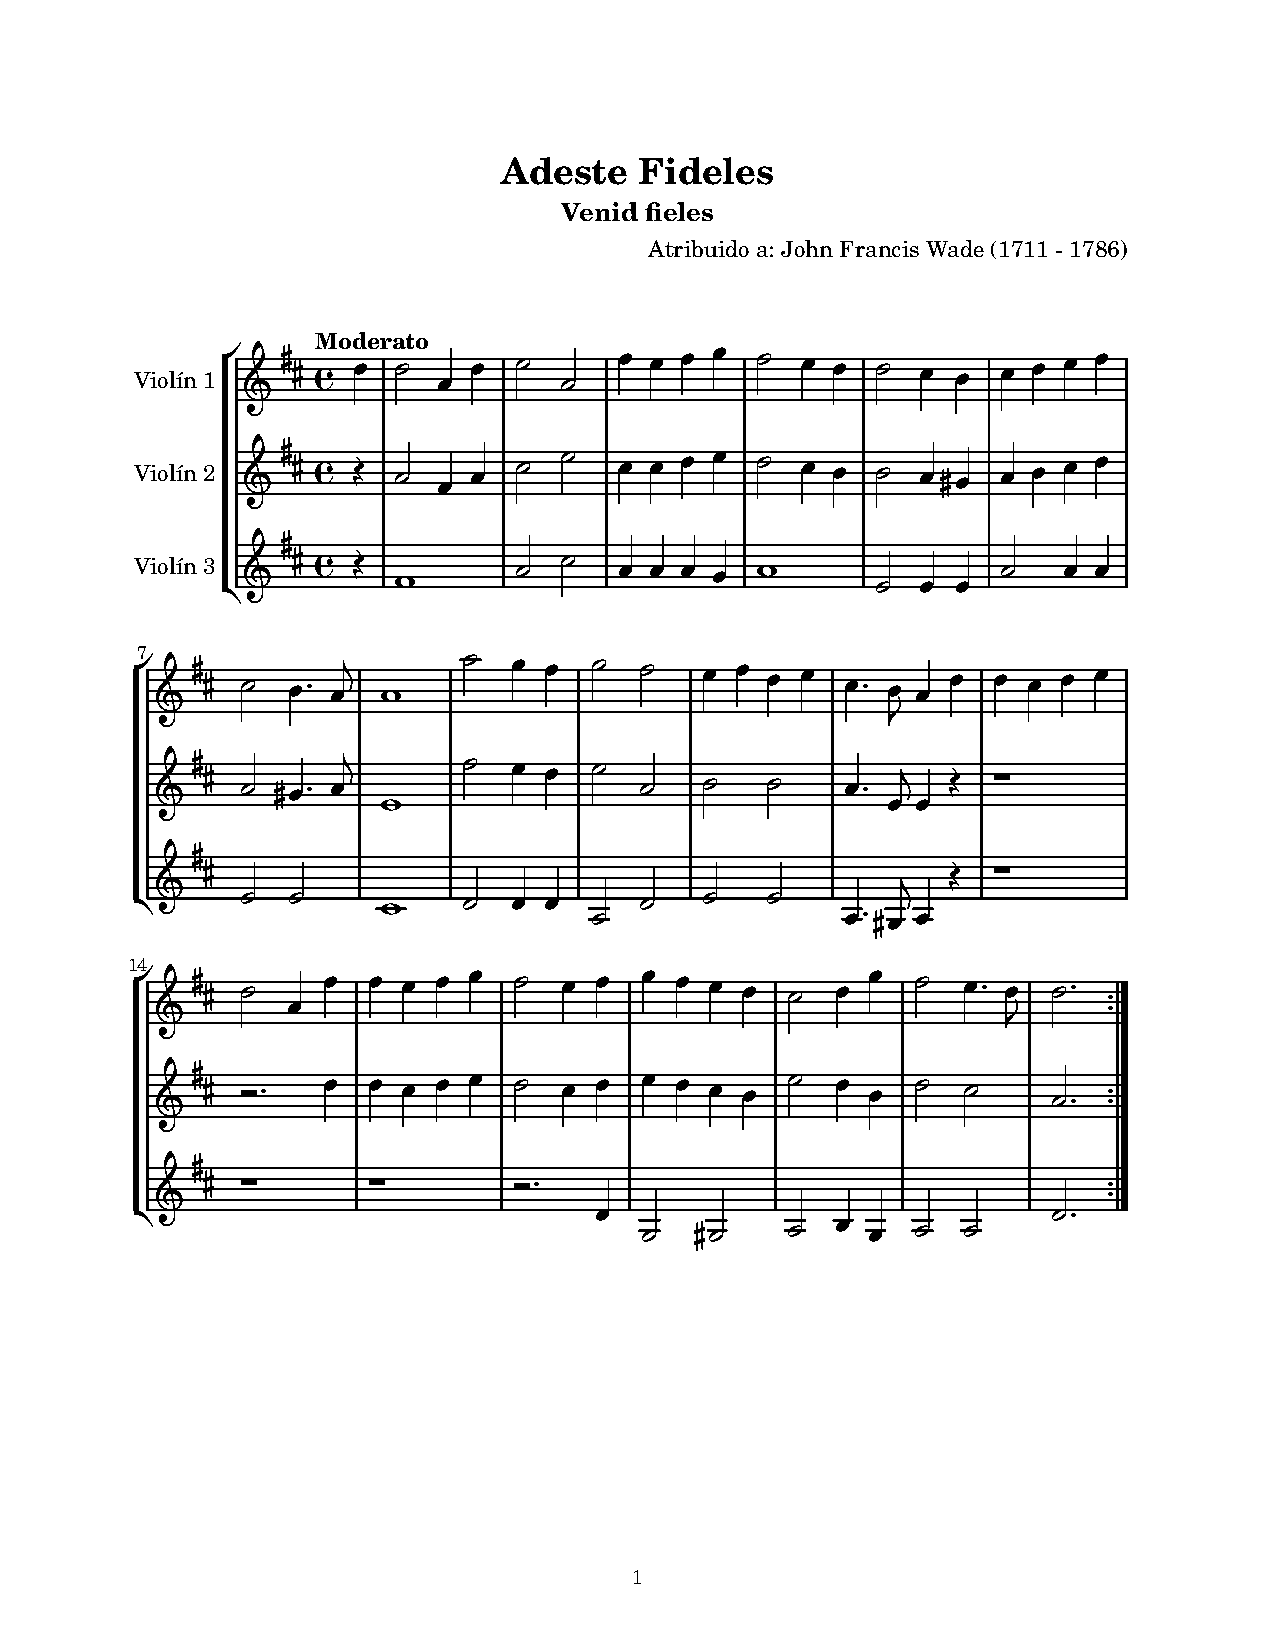
\includepdf[pages=-,addtotoc={
    1,chapter,1,Adeste Fideles,v1,
    2,chapter,1,Noche de Paz,v2,
    3,chapter,1,Campanas de Belén,v3, 
    4,chapter,1,Dime Niño,v4,
    6,chapter,1,{Fum, fum, fum},v5,
    8,chapter,1,Pero mira como beben,v6,
    9,chapter,1,¡Ay del chiquirritin!,v7,
    10,chapter,1,La marimorena,v8,
    11,chapter,1,{Alegría, alegría},v9,
    12,chapter,1,{Rin, rin},v10,
    14,chapter,1,El niño del tambor,v11,
    16,chapter,1,Arre borriquito,v12,
    16,chapter,1,Burrito sabanero,v13,
    16,chapter,1,Suenen las zambombas,v14,
    16,chapter,1,Feliz Navidad,v15,
    17,chapter,1,{Extra: Nearer, My God, to Thee},extra
    }]{../villancicos-compilados.pdf}


\includepdf[pages=-]{../extend/blank.pdf}

\renewcommand{\CoverName}{Colofón}%
\pagestyle{empty}%
\renewcommand{\thepage}{\CoverName}
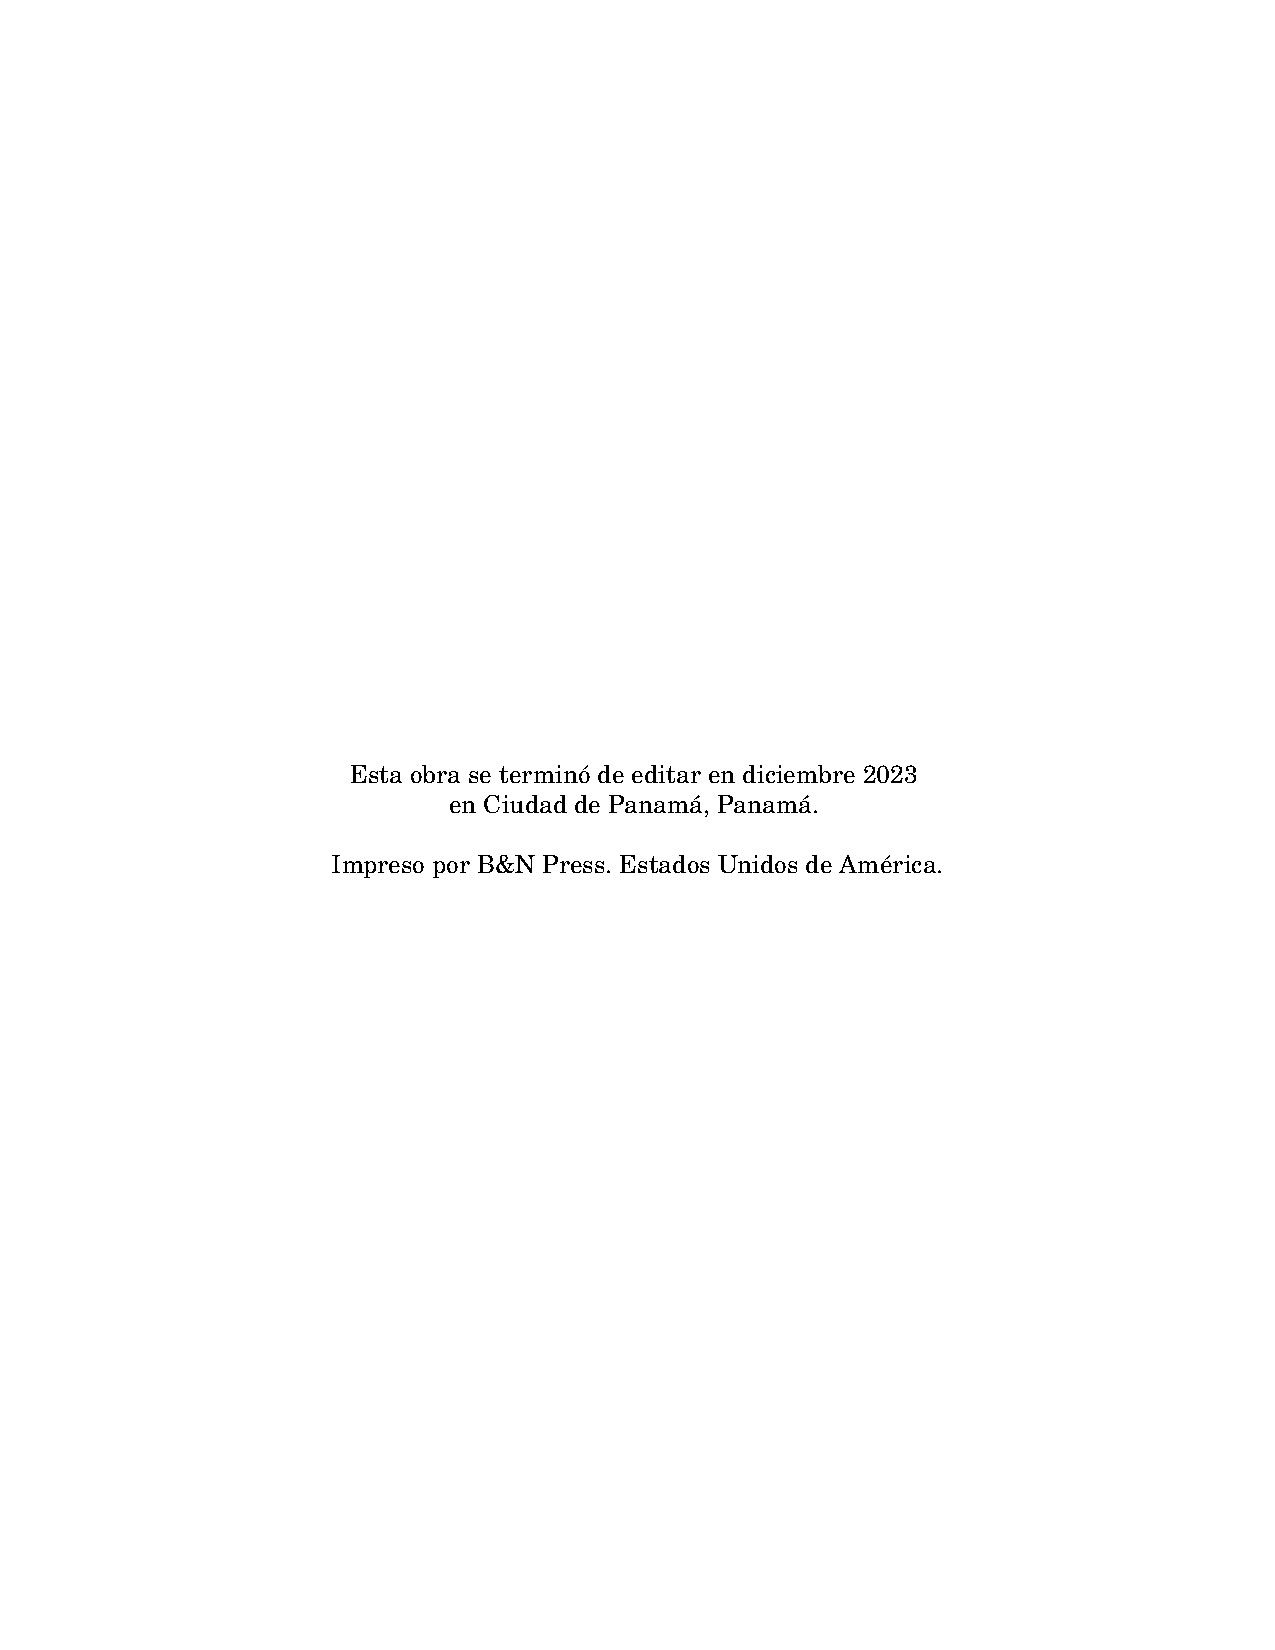
\includepdf[pages=-]{../extend/5-colofon.pdf}

\renewcommand{\CoverName}{Contraportada}%
\pagestyle{empty}%
\renewcommand{\thepage}{\CoverName}
\includepdf{../extend/contraportada.pdf}

\end{document}
